\documentclass[12pt]{article}%
\usepackage{amsfonts}
\usepackage{fancyhdr}
\usepackage{comment}
\usepackage[a4paper, top=2.5cm, bottom=2.5cm, left=2.2cm, right=2.2cm]%
{geometry}
\usepackage{times}
\usepackage{amsmath}
\usepackage{changepage}
\usepackage{amssymb}
\usepackage{float}
\usepackage{graphicx}%
\setcounter{MaxMatrixCols}{30}
\newtheorem{theorem}{Theorem}
\newtheorem{acknowledgement}[theorem]{Acknowledgement}
\newtheorem{algorithm}[theorem]{Algorithm}
\newtheorem{axiom}{Axiom}
\newtheorem{case}[theorem]{Case}
\newtheorem{claim}[theorem]{Claim}
\newtheorem{conclusion}[theorem]{Conclusion}
\newtheorem{condition}[theorem]{Condition}
\newtheorem{conjecture}[theorem]{Conjecture}
\newtheorem{corollary}[theorem]{Corollary}
\newtheorem{criterion}[theorem]{Criterion}
\newtheorem{definition}[theorem]{Definition}
\newtheorem{example}[theorem]{Example}
\newtheorem{exercise}[theorem]{Exercise}
\newtheorem{lemma}[theorem]{Lemma}
\newtheorem{notation}[theorem]{Notation}
\newtheorem{problem}[theorem]{Problem}
\newtheorem{proposition}[theorem]{Proposition}
\newtheorem{remark}[theorem]{Remark}
\newtheorem{solution}[theorem]{Solution}
\newtheorem{summary}[theorem]{Summary}
\newenvironment{proof}[1][Proof]{\textbf{#1.} }{\ \rule{0.5em}{0.5em}}

\newcommand{\Q}{\mathbb{Q}}
\newcommand{\R}{\mathbb{R}}
\newcommand{\C}{\mathbb{C}}
\newcommand{\Z}{\mathbb{Z}}

\begin{document}

\title{CS280 Fall 2021 Assignment 3 \\ Part A}
\author{RNN, LSTM and GRU}
\maketitle

\paragraph{Name: FanYuxin}

\paragraph{Student ID: 2020233216}

\newpage


\subsubsection*{1. Parity-check network (16 points)}
Note that the initial parity bit is 1, what's the relation between each input and the previous parity bit? Determine the relation between the parity and inputs and complete the parity bits($p_1,p_2,p_3,p_4$) and design and draw a RNN to predict parity. 
	
	\begin{align*}
	    \textit{Parity bits}&:\quad\quad0\quad0\quad0\quad1\quad0\quad1\quad p_1\quad p_2\quad p_3 \quad p_4 \quad\rightarrow \\
	    \textit{Input}&:\quad\quad0\quad1\quad1\quad0\quad0\quad0\quad1\qquad1\quad0\qquad0
	\end{align*}

\begin{itemize}
	\item $(p1, p2, p3, p4) = (1, 1, 0,  1)$.
	\item let input as In$_i$ and parity bit as P$_i$. P$_i$ = (P$_{i-1}$ == In$_i$).
	\item RNN: 
	$\mathbf{H}_t = \phi(\mathbf{X}_t \mathbf{W}_{xh} + \mathbf{H}_{t-1} \mathbf{W}_{hh}  + \mathbf{b}_h)$.
	
	$\mathbf{O}_t = \mathbf{H}_t \mathbf{W}_{hq} + \mathbf{b}_q$

	Figure as :
	\begin{figure}[H]
		\centering
		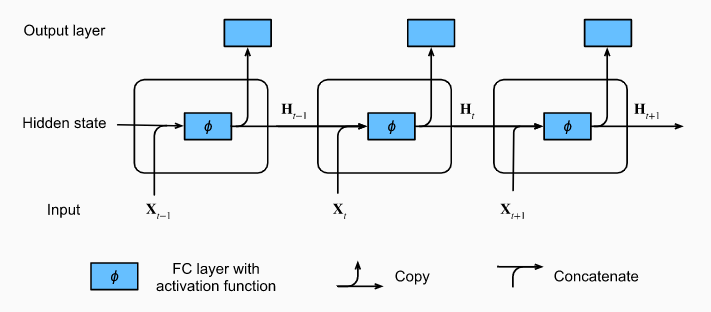
\includegraphics[width=0.9\textwidth]{rnn.png}
	\end{figure}
	
	
	with input demision = 1, hidden size = 2
\end{itemize}

\newpage


\subsubsection*{2. GRU (17 points)}

1. Draw the diagram of GRU, describe the gates (where? What is the role of each gate?), and point out the differences between GRU and LSTM in the design of gates.\\
2. In what situations(s) is LSTM/GRU used respectively? Explain your reason.
\begin{enumerate}
	\item GRU diagram

	\begin{figure}[H]
		\centering
		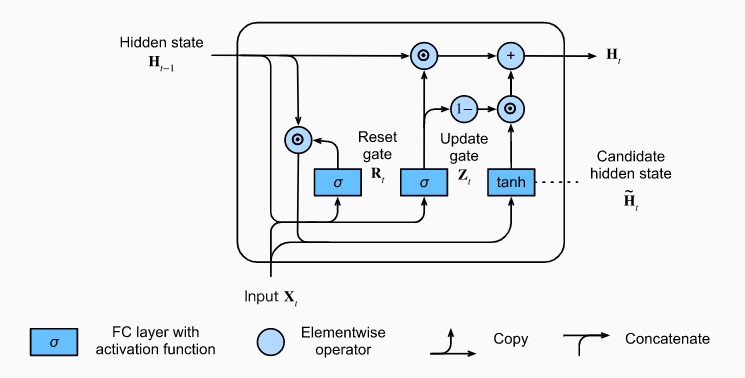
\includegraphics[width=0.85\textwidth]{./gru.png}
	\end{figure}
	Reset gates help capture short-term dependencies in sequences.

	Update gates help capture long-term dependencies in sequences.

	LSTMs have three types of gates: input gates, forget gates, and output gates that control the flow of information.
	The positions of gates of LSTM and GRU are also different.
	\item   
	The number of parameters of GRU is smaller than LSTM. So GRU converges faster than LSTM. 

	When dataset size is small, GRU and LSTM have similar performace, but GRU converges faster. GRU is better.  
	
	When the dataset size is large, LSTM performs better than GRU.
\end{enumerate}


\newpage



\end{document}